%%%%%%%%%%%%%%%%%%%%%%%%%%%%%%%%%%%%%%%%%
% Lachaise Assignment
% LaTeX Template
% Version 1.0 (26/6/2018)
%
% This template originates from:
% http://www.LaTeXTemplates.com
%
% Authors:
% Marion Lachaise & François Févotte
% Vel (vel@LaTeXTemplates.com)
%
% License:
% CC BY-NC-SA 3.0 (http://creativecommons.org/licenses/by-nc-sa/3.0/)
% 
%%%%%%%%%%%%%%%%%%%%%%%%%%%%%%%%%%%%%%%%%

%----------------------------------------------------------------------------------------
%	PACKAGES AND OTHER DOCUMENT CONFIGURATIONS
%----------------------------------------------------------------------------------------

\documentclass{article}

\usepackage{soul}
\sethlcolor{lightgray}

%%%%%%%%%%%%%%%%%%%%%%%%%%%%%%%%%%%%%%%%%
% Lachaise Assignment
% Structure Specification File
% Version 1.0 (26/6/2018)
%
% This template originates from:
% http://www.LaTeXTemplates.com
%
% Authors:
% Marion Lachaise & François Févotte
% Vel (vel@LaTeXTemplates.com)
%
% License:
% CC BY-NC-SA 3.0 (http://creativecommons.org/licenses/by-nc-sa/3.0/)
% 
%%%%%%%%%%%%%%%%%%%%%%%%%%%%%%%%%%%%%%%%%

%----------------------------------------------------------------------------------------
%	PACKAGES AND OTHER DOCUMENT CONFIGURATIONS
%----------------------------------------------------------------------------------------

\usepackage{amsmath,amsfonts,stmaryrd,amssymb} % Math packages

\usepackage[]{fontawesome5}

\usepackage[hidelinks]{hyperref}

\usepackage{enumerate} % Custom item numbers for enumerations

\usepackage[ruled]{algorithm2e} % Algorithms

\usepackage[framemethod=tikz]{mdframed} % Allows defining custom boxed/framed environments

\usepackage{listings} % File listings, with syntax highlighting
\lstset{
	basicstyle=\ttfamily, % Typeset listings in monospace font
}

\usepackage{booktabs} 
\usepackage{colortbl} 
\usepackage{xcolor} 
\usepackage{xfrac}

\newcommand{\ra}[1]{\renewcommand{\arraystretch}{#1}}

%----------------------------------------------------------------------------------------
%	DOCUMENT MARGINS
%----------------------------------------------------------------------------------------

\usepackage{geometry} % Required for adjusting page dimensions and margins

\geometry{
	paper=a4paper, % Paper size, change to letterpaper for US letter size
	top=2.5cm, % Top margin
	bottom=3cm, % Bottom margin
	left=2.5cm, % Left margin
	right=2.5cm, % Right margin
	headheight=14pt, % Header height
	footskip=1.5cm, % Space from the bottom margin to the baseline of the footer
	headsep=1.2cm, % Space from the top margin to the baseline of the header
	%showframe, % Uncomment to show how the type block is set on the page
}

%----------------------------------------------------------------------------------------
%	FONTS
%----------------------------------------------------------------------------------------

\usepackage[utf8]{inputenc} % Required for inputting international characters
\usepackage[T1]{fontenc} % Output font encoding for international characters

\usepackage{XCharter} % Use the XCharter fonts

%----------------------------------------------------------------------------------------
%	COMMAND LINE ENVIRONMENT
%----------------------------------------------------------------------------------------

% Usage:
% \begin{commandline}
%	\begin{verbatim}
%		$ ls
%		
%		Applications	Desktop	...
%	\end{verbatim}
% \end{commandline}

\mdfdefinestyle{commandline}{
	leftmargin=10pt,
	rightmargin=10pt,
	innerleftmargin=15pt,
	middlelinecolor=black!50!white,
	middlelinewidth=2pt,
	frametitlerule=false,
	backgroundcolor=black!5!white,
	frametitle={Command Line},
	frametitlefont={\normalfont\sffamily\color{white}\hspace{-1em}},
	frametitlebackgroundcolor=black!50!white,
	nobreak,
}

% Define a custom environment for command-line snapshots
\newenvironment{commandline}{
	\medskip
	\begin{mdframed}[style=commandline]
}{
	\end{mdframed}
	\medskip
}

%----------------------------------------------------------------------------------------
%	FILE CONTENTS ENVIRONMENT
%----------------------------------------------------------------------------------------

% Usage:
% \begin{file}[optional filename, defaults to "File"]
%	File contents, for example, with a listings environment
% \end{file}

\mdfdefinestyle{file}{
	innertopmargin=1.6\baselineskip,
	innerbottommargin=0.8\baselineskip,
	topline=false, bottomline=false,
	leftline=false, rightline=false,
	leftmargin=2cm,
	rightmargin=2cm,
	singleextra={%
		\draw[fill=black!10!white](P)++(0,-1.2em)rectangle(P-|O);
		\node[anchor=north west]
		at(P-|O){\ttfamily\mdfilename};
		%
		\def\l{3em}
		\draw(O-|P)++(-\l,0)--++(\l,\l)--(P)--(P-|O)--(O)--cycle;
		\draw(O-|P)++(-\l,0)--++(0,\l)--++(\l,0);
	},
	nobreak,
}

% Define a custom environment for file contents
\newenvironment{file}[1][File]{ % Set the default filename to "File"
	\medskip
	\newcommand{\mdfilename}{#1}
	\begin{mdframed}[style=file]
}{
	\end{mdframed}
	\medskip
}

%----------------------------------------------------------------------------------------
%	NUMBERED QUESTIONS ENVIRONMENT
%----------------------------------------------------------------------------------------

% Usage:
% \begin{question}[optional title]
%	Question contents
% \end{question}

\mdfdefinestyle{question}{
	innertopmargin=1.2\baselineskip,
	innerbottommargin=0.8\baselineskip,
	roundcorner=5pt,
	nobreak,
	singleextra={%
		\draw(P-|O)node[xshift=1em,anchor=west,fill=white,draw,rounded corners=5pt]{%
		Question \theQuestion\questionTitle};
	},
}

\newcounter{Question} % Stores the current question number that gets iterated with each new question

% Define a custom environment for numbered questions
\newenvironment{question}[1][\unskip]{
	\bigskip
	\stepcounter{Question}
	\newcommand{\questionTitle}{~#1}
	\begin{mdframed}[style=question]
}{
	\end{mdframed}
	\medskip
}

%----------------------------------------------------------------------------------------
%	WARNING TEXT ENVIRONMENT
%----------------------------------------------------------------------------------------

% Usage:
% \begin{warn}[optional title, defaults to "Warning:"]
%	Contents
% \end{warn}

\mdfdefinestyle{warning}{
	topline=false, bottomline=false,
	leftline=false, rightline=false,
	nobreak,
	singleextra={%
		\draw(P-|O)++(-0.5em,0)node(tmp1){};
		\draw(P-|O)++(0.5em,0)node(tmp2){};
		\fill[black,rotate around={45:(P-|O)}](tmp1)rectangle(tmp2);
		\node at(P-|O){\color{white}\scriptsize\bf !};
		\draw[very thick](P-|O)++(0,-1em)--(O);%--(O-|P);
	}
}

% Define a custom environment for warning text
\newenvironment{warn}[1][Warning:]{ % Set the default warning to "Warning:"
	\medskip
	\begin{mdframed}[style=warning]
		\noindent{\textbf{#1}}
}{
	\end{mdframed}
}

%----------------------------------------------------------------------------------------
%	INFORMATION ENVIRONMENT
%----------------------------------------------------------------------------------------

% Usage:
% \begin{info}[optional title, defaults to "Info:"]
% 	contents
% 	\end{info}

\mdfdefinestyle{info}{%
	topline=false, bottomline=false,
	leftline=false, rightline=false,
	nobreak,
	singleextra={%
		\fill[black](P-|O)circle[radius=0.4em];
		\node at(P-|O){\color{white}\scriptsize\bf i};
		\draw[very thick](P-|O)++(0,-0.8em)--(O);%--(O-|P);
	}
}

% Define a custom environment for information
\newenvironment{info}[1][Info:]{ % Set the default title to "Info:"
	\medskip
	\begin{mdframed}[style=info]
		\noindent{\textbf{#1}}
}{
	\end{mdframed}
}
 % Include the file specifying the document structure and custom commands

%----------------------------------------------------------------------------------------
%	ASSIGNMENT INFORMATION
%----------------------------------------------------------------------------------------

\title{Embedded Systems \\ \textsc{OpenWrt} WiFi Multi-Channel Sniffer} % Title of the assignment

\author{Giovanni Baccichet \\ \raisebox{0.1\height}{\fontsize{8}{8}\faUser} \texttt{10851745}} % Author name and email address

\date{Politecnico di Milano --- \today} % University, school and/or department name(s) and a date

%----------------------------------------------------------------------------------------

\begin{document}

\maketitle % Print the title

%----------------------------------------------------------------------------------------
%	INTRODUCTION
%----------------------------------------------------------------------------------------

\section{Introduction} % Unnumbered section

\begin{warn}[External Resources]
    Everything disclosed in this report (except for the network dumps, due to privacy reasons) can be found in this repository: \href{https://github.com/GiovanniBaccichet/openwrt-multi-sniffer}{\raisebox{0.1\height}{\fontsize{8}{8}\faLink} github.com/GiovanniBaccichet/openwrt-multi-sniffer}.
\end{warn}

The ever-increasing integration of wireless technology into our everyday lives brings with it a spectrum of challenges and opportunities. One such opportunity resides in the analysis of WiFi probe request frames which are inherently broadcasted by WiFi-enabled devices as they search for available networks. By performing a detailed analysis of these frames, we can gain insightful knowledge about the device behavior, network congestion, security aspects, and much more.

This project aims to harness this potential by utilizing off-the-shelf hardware in combination with OpenWrt, a leading open-source router Operating System (OS). The primary goal is to develop a cost-effective and efficient system for \textbf{WiFi Probe Request frame sniffing over multiple channels}, specifically focusing on the 2.4 GHz and 5 GHz spectrum bands, traditionally used in WiFi communications. 

Leveraging the inherent power and flexibility of OpenWrt, the system will be capable of capturing and analyzing WiFi Probe Request frames, thereby providing an accessible, in-depth perspective on the wireless activity in a given environment. This data can be crucial in a variety of scenarios, from troubleshooting network issues, cybersecurity investigations, to academic research, and more.

The system's functionality will be presented through \textsc{OpenWrt}'s LuCi web graphical user interface (GUI), where users can view real-time data, and manage the overall operation. The user-friendly interface ensures that even those with little to no technical background can easily use the system. The collected data can be stored locally, offering an opportunity for subsequent detailed analysis or long-term trend observation.

This innovative approach combines the power of open-source software with the availability and affordability of consumer hardware, opening doors for a new kind of WiFi network analysis tool. This system has vast potential for a wide array of applications, such as network performance optimization, device tracking, studying human behavior through device movement, and contributing towards the broader fields of IoT and Smart Cities.

%----------------------------------------------------------------------------------------
%	IEEE 802.11 RECALL
%----------------------------------------------------------------------------------------


\section{Background on IEEE 802.11}

\begin{info}[Active Scanning]
    Active scanning is a proactive method employed by wireless devices, or stations, to identify Wi-Fi networks within their proximity.
\end{info}

When a device is set to actively scan, it releases a frame called a "Probe Request". This is the station's way of declaring its presence and asking nearby networks to respond. There are two types of probe requests: a broadcast probe, which is a general call-out to any network within range, and a directed probe, which is specifically aimed at a particular network identified by its Service Set Identifier (SSID).

Upon receiving a probe request, any access point (AP) within range responds with a "Probe Response" frame. This frame isn't simply an acknowledgement; it also serves as an information packet that carries specifics about the network. These specifics include the SSID, data rates that the network can support, the specific 802.11 physical layer (PHY) standard in use (like 802.11ac, 802.11n), channel usage, and much more. 

\begin{figure}[h]
    \centering
    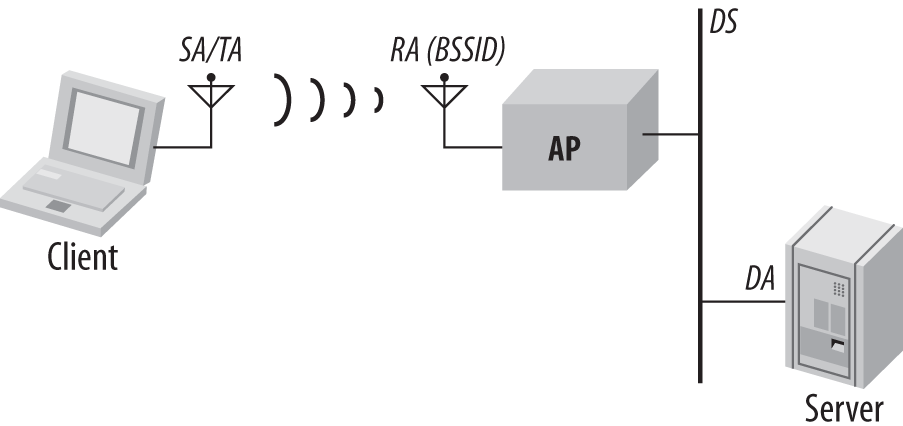
\includegraphics[width=0.55\textwidth]{assets/address-field-usage.png}
    \caption{Address Field Usage in WiFi Networks}
    \label{fig:address-field}
\end{figure}

Having collected the probe responses from all APs within range, the station then has the task of selecting the most suitable network to join. This decision isn't just influenced by signal strength, but also factors in aspects like network congestion, supported security protocols, and others. 

Zooming in on the probe request frame, one realizes that it's a container for a wealth of information. Most notably, it carries the source MAC address - a unique identifier attached to the device's network interface card (NIC). Traditionally, each NIC has a globally unique MAC address.

\begin{figure}[h]
    \centering
    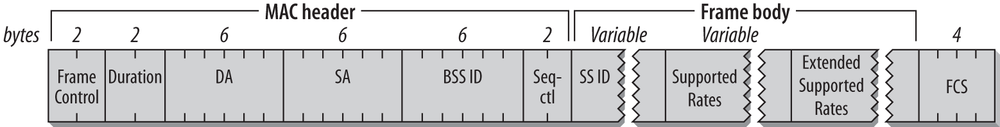
\includegraphics[width=0.7\textwidth]{assets/probe-request-frame.png}
    \caption{Probe Request Frame}
    \label{fig:probe-request-frame}
\end{figure}

This MAC address uniqueness has a flip side: it creates a potential privacy risk because the consistent use of a static MAC address allows for tracking of the device. To mitigate this risk, many modern devices employ a technique known as MAC address randomization. With this approach, the MAC address that the device uses to communicate on the network isn't static but changes periodically. Thus, even if a probe request is intercepted and the MAC address logged for tracking, the address would have changed by the next cycle, adding a layer of privacy protection.

However, while MAC address randomization helps, it is not a foolproof solution. Certain patterns in the randomization process or additional identifiable information in the probe requests may still enable tracking or identification of the device. Therefore, the evolution and robustness of privacy-protection mechanisms like MAC address randomization remain a topic of ongoing research and development. 

With wireless communication becoming even more widespread, the interplay between technology, data analytics, privacy, and cybersecurity becomes ever more complex and intriguing. The continuous study of these facets within the realm of Wi-Fi probe request tracking is, thus, a pressing and compelling necessity.

%------------------------------------------------

\section{Infrastructure Overview}

The infrastructure for this project was designed with careful consideration to ensure optimal performance, robustness, and ease of use. We leveraged the capabilities of the \texttt{Linksys MR8300 v1.1} as the primary hardware component for our setup. This device is an advanced MU-MIMO Tri-Band WiFi router known for its superior performance and flexible functionality.

\begin{figure}[h]
    \centering
    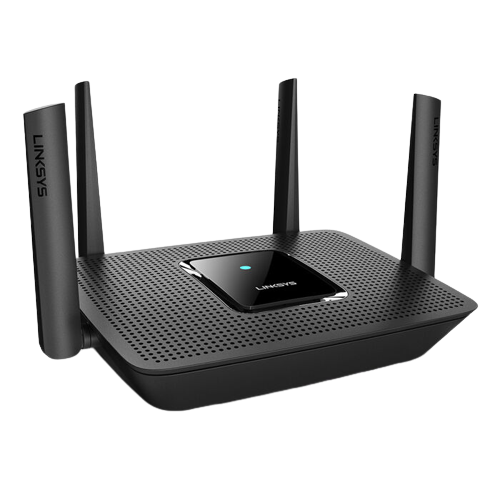
\includegraphics[width=0.4\textwidth]{assets/linksys_mr800.png}
    \caption{Linksys MR8300 Router}
    \label{fig:router}
\end{figure}

Running on \texttt{\textsc{OpenWrt} 22.03.2}, an open-source router operating system renowned for its stability and community support, the Linksys MR8300 allows us to implement and execute our WiFi probe request frame sniffing system smoothly. The OS's open nature provides us with the flexibility to modify and tweak the system as per our requirements.

The Linksys MR8300 comes with one 2.4GHz WiFi interface and two 5GHz WiFi interfaces, enabling us to cover the entire range of commonly used WiFi spectrum bands. This wide spectrum coverage is vital for our system to monitor and analyze WiFi probe request frames across multiple channels effectively.

One of the primary reasons we chose the Linksys MR8300 was its generous hardware specifications, making it highly suitable for data-intensive operations. It is equipped with 512 MB of RAM and 256 MB of NAND ROM, providing ample space for storing and processing data. Additionally, the powerful \texttt{Qualcomm IPQ4019} CPU ensures efficient processing and seamless operation of the system.

Moreover, the Linksys MR8300 boasts four 1 Gbps LAN ports and one 1 Gbps WAN port, allowing for high-speed, wired connections when needed. The USB 3.0 interface opens up possibilities for additional storage or other peripherals, and the four external antennas ensure excellent wireless coverage. Additionally, the device includes a Bluetooth chip, which could be utilized for other projects or applications.

The support and community around this device are robust, ensuring that any issues can be addressed swiftly and effectively. Its advanced features and capabilities make it a suitable choice for similar projects and applications, promoting flexible and powerful network solutions. Overall, the Linksys MR8300 running \textsc{OpenWrt} provides a solid foundation for our system's setup.

\subsection{Remote File Storage}

In addition to the already mentioned setup, there is potential to employ tunneling solutions such as Tailscale to transfer data to a remote network filesystem. This technology allows secure connections to be established over the internet, effectively creating a virtual network infrastructure that can span across multiple geographical locations.

Tailscale is a secure network connectivity tool that leverages WireGuard, a modern, high-performance VPN protocol. It is renowned for its simplicity, speed, and security. With Tailscale, you can create a virtual private network (VPN) that connects your device to a remote network, even across NAT, firewalls, or other restrictive network environments.

In the context of our project, Tailscale can be used to securely send the collected WiFi probe request frame data from our \textsc{OpenWrt}-based device to a remote network filesystem. This could be especially useful when the system is deployed in a remote or difficult-to-access location, or if you want to aggregate data from multiple devices into a central storage location for further analysis.

This remote network filesystem could be a dedicated Network Attached Storage (NAS) system, a server, or even a cloud-based storage service. The data can then be accessed, analyzed, and managed remotely, providing an extra layer of convenience and flexibility.

Using Tailscale or similar solutions, the data captured by our system can be transmitted securely and reliably over the internet, allowing for remote data analysis and storage. This extends the use cases for our project, making it even more versatile and effective for a wide range of applications.

\section{Methodology}

For the core functionality of sniffing WiFi probe requests, we leveraged two important tools: \texttt{tcpdump} and \texttt{iw}. \texttt{tcpdump} is a robust command-line packet analyzer, while \texttt{iw} is a flexible tool used for configuring Linux wireless devices. By integrating these tools, we ensured efficient and accurate data capture from the WiFi environment, using stat-of-the-art tools.

We then developed a shell script that uses these tools to put all wireless interfaces into monitor mode, which is a mode that allows WiFi devices to listen to all frames on the network. Following this, we used \texttt{tcpdump} to capture the management frames, specifically probe request frames. These frames are sent out by devices seeking to connect to WiFi networks, and they contain valuable information such as MAC address, RSSI (Received Signal Strength Indicator), and timestamp. 

To make the data more consumable, we parsed the output from \texttt{tcpdump} to extract these data fields and formatted them in a JSON structure. The JSON format was chosen because of its wide acceptance and ease of use in data handling, particularly for web-based user interfaces. 

Finally, we built a module in LuCI to display this information. A new page was created to present the data in a tabular form, with columns for each data field including MAC address, vendor, channel, RSSI, and timestamp. By using Lua scripting, we were able to manipulate the JSON data and render it effectively in the LuCI interface. 

Throughout this process, we consistently prioritized the selection and use of open-source and widely-used tools, enabling future adaptability and extensibility of the project. We strived to ensure efficient data capture, processing, and presentation, all contributing to the final goal of providing a robust and user-friendly WiFi probe request sniffer.


\section{Results}
 
Here is the results, include screenshots and code snippets.


%----------------------------------------------------------------------------------------

\end{document}
